\section{Experimental systems}\label{sec:experimental}

Both datasets of this section come from magnetic reservoir-computing hardware rather than from simulation. Neither system has a governing equation we trust enough to integrate numerically, which is precisely the regime the package targets. The trained surrogate therefore consumes the output of the raw measurement pipeline, subject only to the light preprocessing described below.

The same forward corruption, conditional denoiser and deterministic DDIM sampler developed through the OU example apply without change. The experimental cases differ only in their preprocessing, representation and conditioning design. 

\begin{figure}[h!]\centering
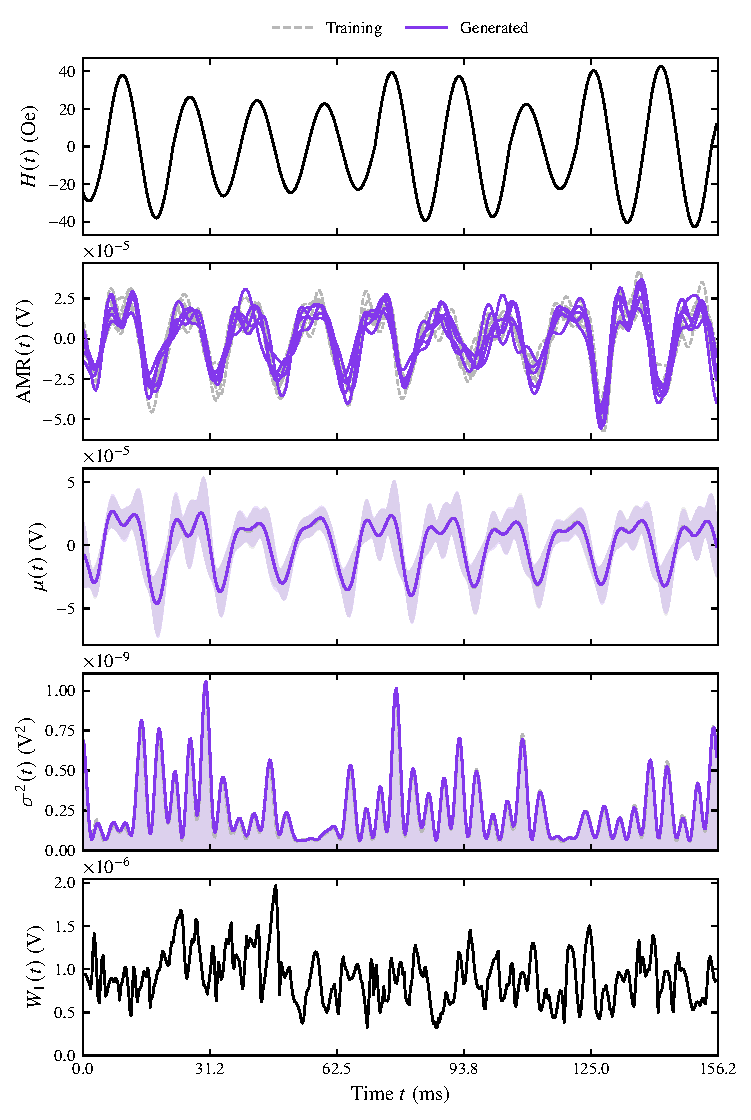
\includegraphics[width=0.9\linewidth]{amr.pdf}
\caption{}
\label{fig:amr}
\end{figure}

\subsection{Magnetoresistance with full-waveform conditioning}\label{ssec:amr}

The first dataset comprises magnetisation dynamics from an experimental spintronic device consisting of a lithographically patterned, interconnected array of permalloy
$\mathrm{Ni}_{80}\mathrm{Fe}_{20}$ nanoscale rings.  The array is driven by an in-plane rotating magnetic field with amplitude $H(t)$, and the resulting anisotropic magnetoresistance (AMR) is measured.\footnote{These dynamics provide the nonlinearity and fading memory required for reservoir computing~\cite{dawidek2021,vidamour2022,manneschi2025}.}  We refer the reader to Ref.~\cite{manneschi2025} for details of the device and measurement procedure.

Each AMR channel is modelled separately.  A training example is
\[
\left(\mathbf{q}^{(i)},\mathbf{h}^{(i)}\right),
\qquad
\mathbf{q}^{(i)},\mathbf{h}^{(i)}\in\mathbb{R}^{N_T},
\qquad
N_T=5000,
\]
where $\mathbf{q}^{(i)}$ is the measured AMR trajectory and $\mathbf{h}^{(i)}$ is the corresponding discretised field-amplitude waveform.  The raw measurements contain $100$ repetitions of each of $999$ field patterns.  After removing acquisition transients, each trajectory contains $5000$ samples, corresponding to $100$ cycles of $50$ samples at a sampling rate of $3200\,\mathrm{Hz}$.  The AMR is filtered using a fifth-order, zero-phase Butterworth band-pass filter from $40$ to $200\,\mathrm{Hz}$.  The field amplitude is represented as a stepwise conditioning signal, with one normalised value held constant over each $50$-sample cycle.  Ten repetitions per pattern are used, and the patterns are divided into training, validation, and test sets in an $80{:}10{:}10$ ratio. 

The conditional U-Net has hidden width $64$, kernel size $3$, and dilation factors $(1,2,4,8)$. The dilation schedule gives an effective receptive field of approximately $19$ field cycles, or $329\,\mathrm{ms}$, allowing the model to represent the long-range temporal correlations and coloured noise in the AMR signal. The trajectory length $N_T=5000$ is independent of the $1000$ algorithmic diffusion steps used during training.  The model is trained with noise-prediction mean-squared error and sampled using DDIM.

\subsection{Diffusion modelling of spectrograms: artificial spin ice}\label{ssec:asi}

The second dataset is obtained from an artificial-spin-ice (ASI) multilayer reservoir probed by ferromagnetic resonance (FMR) spectroscopy \cite{stenning2024neuromorphic}. The applied field, $H_{\mathrm{app}}(t)$, varies between approximately $180$ and $235\,\mathrm{mT}$, following either a Mackey--Glass or sinusoidal waveform. The measured response is $\mathrm{d}P/\mathrm{d}H$, recorded in arbitrary units across $N_F=201$ fixed frequency bins. Each trajectory is therefore a time--frequency matrix $\mathbf{Y}^{(i)}\in\mathbb{R}^{T\times201}$. The data were separated into experimental runs, divided into $T=50$-step windows with stride $10$, and split at the run level. This produced $359$ training and $84$ test windows for Mackey--Glass, and $448$ training and $104$ test windows for the sine wave. The field was globally $z$-scored, and each FMR channel was normalised using its training mean and standard deviation.

The data supplied to the diffusion model are multivariate one-dimensional time series. PCA was fitted to the training matrices after reshaping (from $[N_{\mathrm{train}},T,201]$ to $[N_{\mathrm{train}}T,201]$), so that each time slice was one observation and the frequency bins were the features. After mode-wise normalisation, the trajectories were rearranged to shape $K\times T$. We use $K=16$ modes, which explain $96.9\%$ of the Mackey--Glass variance.

The diffusion model receives these PCA modes and is conditioned on the input field. A one-dimensional residual U-Net convolves along the time axis; the 16 PCA modes are treated as jointly generated channels. The U-Net has three levels of dilation: $[1,2,4]$. The PCA is then inverted to reconstruct the full spectrogram.

This representation is suited to the available data. The Mackey--Glass training set contains only $359$ windows from $15$ experimental runs, and the stride-$10$ windows overlap. A two-dimensional image model would learn directly in the $50\times201=10{,}050$-value time--frequency space, with convolutions across both time and frequency. The PCA representation reduces the generated state to $16\times50=800$ values, which may capture the global correlations between the fixed frequency channels, and allows the U-Net to focus on temporal dynamics. It therefore provides a more data-efficient model for this small experimental dataset while retaining the full frequency response through inverse PCA. We observe that increasing the number of retained principal components beyond $K=64$ deteriorates training, for reasons we do not yet understand.